\documentclass[preprint,12pt]{elsarticle}
\usepackage{courier}
%Author: Adam Duby, UCCS

% Advisor:
% Yanyan Zhuang (Operating Systems and Software Engineering)

% Committee Members:
% Edward Chow (Engineering Security)
% Jason Upchuch (Malware Forensics and Reverse Engineering)
% Qing Yi (Compilers)

\usepackage{graphicx}
\usepackage{amssymb}
\usepackage{lineno}
\journal{UCCS, Department of Computer Science}

\begin{document}
\begin{frontmatter}

\title{A Survey on Software Diversification and Deception\\\large A Survey for Completing the PhD Qualifying Exam Requirement}

\author{Adam Duby}
\address{Department of Computer Science\\University of Colorado Colorado Springs\\Colorado Springs, CO\\
\ead{aduby@uccs.edu}}

\begin{abstract}
Software diversification continues to be active research topic in the Moving Target Defense (MTD) community. Despite the volume of research activity, the only diversification scheme that has enjoyed widespread deployment is address space layout randomization (ASLR). The goal of diversification is to thwart memory disclosure vulnerabilities that can lead to code reuse and code injection attacks. Semantically equivalent, yet syntactically unique instances of software diversifies the attack surface. This creates a deceptive and unpredictable execution environment for malicious code while reducing attack scalability and the exposure of existing vulnerabilities. 

In this paper, we examine diversification at various layers, including compiler-generated diversity and operating system interface diversification. We also address the potential for software deception in conjunction with code diversification as a defense. Deception provides the attacker with enticing code gadgets, that when triggered serve as a tripwire to alert the defense of an active code reuse attack. We discuss the influential work in these fields and suggest some potential open research problems and improvements for future work. This paper also addresses the less documented problem of re-purposed code diversification routines by malicious actors to defeat static signatures and similarity comparisons for malware classification. Current literature offers studies in static comparisons, but there is a lack of work on the effectiveness of static similarity against an explicitly diversified set of samples.
\end{abstract}
\end{frontmatter}

%% main text
\section{Introduction}
\label{S:1}

Since the widespread adoption of Data Execution Prevention (DEP) and Address Space Layout Randomization (ASLR) \cite{team2003pax}, attackers have modified their exploitation tactics from traditional code injection to advanced code reuse attacks. Code reuse enables attackers to bypass DEP since they no longer depend on injecting executable shellcode on the stack. Attackers realized that existing code already mapped to executable code pages can be re-purposed for malicious endeavors. Software security researchers have responded with increased research efforts to thwart these attacks.

This response triggered the code diversification and randomization paradigm. In order for an attacker to build a successful code reuse attack, they rely on code information from the victim process. Attackers can perform offline analysis and reverse engineering to learn how to restructure the benign program's control flow to achieve malicious effects. Further, attacks are easily scalable across multiple target sets with minimal additional cost due the monoculture in the software landscape. For example, if a software application is exploitable, then every instance of that same software is exploitable. Diversification and randomization eliminates the stasis and predictability that is afforded to the offense by the defensive monoculture. A malleable and diversified terrain will increase the complexity and cost of attacks while reducing attack scalability. If the diversification is random and continuous over time, it provides an unpredictable attack surface and reduces the exposure of vulnerabilities. An attacker conducting reconnaissance and enumeration will not have intelligence valuable for any significant length of time, denying them the advantage of time to plan and coordinate the attack. It can also reduce the duration of persistent adversary access by denying the adversary an execution environment compatible with the attack tools and techniques.

Efficient and effective randomization relies on the assumption of memory secrecy. However, new information disclosure attacks that bypass randomization through return oriented programming (ROP) attacks are being published in response to almost every proposed code diversification technique \cite{strackx2009breaking}\cite{snow2013just}\cite{schuster2015counterfeit}\cite{bletsch2011jump}\cite{rudd2017address}\cite{shacham2007geometry}\cite{bittau2014hacking}. This class of attacks is proving challenging to completely mitigate through code diversification. Thus, operating system randomization and control flow integrity (CFI) research has been complementing the search for effective defenses.

Operating system randomization and diversification is not a new concept. Defenses through operating system code diversification \cite{cohen1993operating} and address space randomization \cite{team2003pax} has been in literature for decades. However, more aggressive randomization schemes are now being proposed to render the execution environment incompatible with malware \cite{Rauti14}\cite{rauti2018internal}\cite{rauti2014towards}\cite{srivastava2008system}\cite{jiang2007randsys}\cite{giuffrida2012enhanced}\cite{chew2002mitigating}. 

Attackers can also use code randomization to defeat signatures and similarity testing \cite{payer2014embracing} \cite{payer2014similarity}. It is not uncommon for malware to utilize polymorphism and code obfuscation, but these techniques can often be detected from their high entropy code sections. Thus, code diversification introduced by the compiler can offer attackers an alternative to obfuscation. Literature suggests both static and dynamic techniques to detect malware variants of the same family. Dynamic analysis tends to focus on system call patterns, while static analysis examines the file structure for similarities. We scope our discussion to static analysis, since their is a lack of research documenting the effectiveness of static similarity techniques on a diversified malware corpus.

The rest of this paper is organized as follows. Section 2 discusses program control flow as it traverses the operating system. We provide a treatment on Windows 10 x64 and Linux x64 as examples. Section 3 provides the threat model. Section 4 summarizes current research for defending against code reuse attacks. Section 5 provides a condensed outline of the key papers we consider for our research. Section 6 proposes several tasks for future work. Section 7 summarizes the paper.

\section{Program Control Flow and Execution Background}
\label{S:2}

In this section, we discuss control flow in program execution. We demonstrate how the flow of control is transferred between function calls and system calls. We also examine linking and loading to demonstrate how library and operating system interface routines are invoked. We specifically look at Windows and Linux implementations.

\subsection{Compilation and Execution}
Software must be compiled into a machine code that is compatible with the underlying architecture. Programs written in higher level languages are the input to the compiler, and executable binary code is the output. The binary output file must also be compatible with the operating system. For example, Windows programs must comply with the Portable Executable (PE) file format, while Linux programs comply with the Executable and Linkable Format (ELF). The compilation process is complex, transformative, and lossy. The compiler parses the source code into tokens via the lexical analyzer. Semantics are then represented through some lower level intermediate representation (IR). The IR is typically architecture agnostic, and used by the compiler to perform optimization. Operating system and architecture specific code generation routines are then performed to produce machine code (object code). This object file is then fed into the compile-time linker, which combines the various source code files together and packages the program into one of the operating system's files formats (PE or ELF).

When executed, the operating system's loader loads the program into memory and creates a process address space. The runtime linker builds a linking table to replace the dynamically linked API calls with pointers to the appropriate external library routine. These dynamically linked shared libraries can provide additional functionality (third-party libraries), and are also used to interface with the operating system. Control flow is managed through the instruction pointer (IP), which is a register that points to the next instruction to execute. The IP is manipulated through call and ret instructions, who use the stack to transfer function parameters and control flow information, such as the return address. User mode programs frequently make traps into kernel mode in order to interface with the operating system. In the following sections, we examine this process in more depth on a Windows 10 and Linux Debian system. We use a combination of reverse engineering tools to follow the execution of some simple programs. This exercise solidified our understand of the underlying mechanics necessary for analyzing the existing literature.

\subsection{Windows Control Flow}

To study the control flow on Windows, we created a simple program, shown in Figure \ref{fig:windowsDemo64.c}, that we compiled using Visual Studios (VS). We use the \texttt{CreateFile} Win32 API call to demonstrate how the Windows linker enables the program to interface with the Windows library and how the loader memory maps shared dynamically linked libraries (DLL) into the process address space. Our sample also demonstrates explicit runtime linking, also known as delay loading, through the use of the \texttt{LoadLibrary} and \texttt{GetProcAddress} functions. Here we will show how to link to a library, in this case a simple custom DLL we called \texttt{myDLL64.dll}, without using the compile-time linker. This is a common technique used by malware to defeat static import library analysis.

\begin{figure}[ht]
\fbox{\centering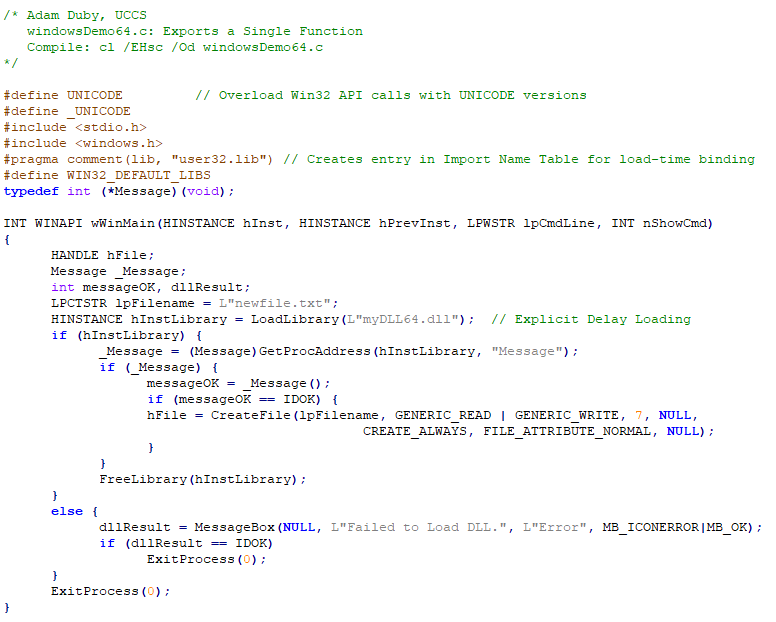
\includegraphics[width=1\linewidth]{Figures/windowsDemo64_c}}
\caption{windowsDemo64.c}
\label{fig:windowsDemo64.c}
\end{figure}

In Figure \ref{fig:windowsDemo64.c}, the program calls the Win32 function \texttt{CreateFile}. This function is defined inside of \texttt{kernel32.dll}. In order to make use of external libraries, the compiler needs to access the library's symbol table. Since all Windows applications load the \texttt{kernel32.dll} library, there is no need to manually include the library in the source code. The program also calls \texttt{MessageBox}, which is defined in \texttt{user32.dll}. Since \texttt{user32.dll} is not automatically loaded, its library file, \texttt{user32.lib}, must be included in the source code. Compiled Windows binaries (.exe and .dll) adhere to the Portable Executable file structure, or the PE32 for 32-bit binaries and PE32+ for 64-bit binaries. During compilation, a section in the PE32 binary called the \texttt{.reloc} section is built to map symbols, certain functions, and direct memory addressing to the appropriate call sites. This enables position independence through relocatable relative virtual addresses (RVAs) and offsets. This also enables ASLR to map the base image of the executable into a random memory page.

The compiler also creates an import directory. The import directory contains an Import Name Table (INT) that contains a list of the names of the dynamically linked DLLs and the exported functions from said DLLs that the program invokes. At compile time, a section is reserved at the end of the program's \texttt{.text} section. This special section, called the \texttt{.idata} section, will be filled in at load time with the addresses of the call sites for the imported functions. When the program is first loaded, the linker and loader make a pass at the program to examine the DLLs in the INT. Those DLLs then get mapped to the process's address space. Then the RVAs in the INT are examined to find where in the \texttt{.idata} section the linker should insert the pointer to the appropriate call site. This list of pointers is called the Import Address Table (IAT). Similarly, DLLs contain an export directory which contains a list of exported functions in an export name table (ENT). The export directory also contains the RVAs of the exported functions' call sites. The load-time linking process resolves a process's IAT by examining the DLL's export directory in order to fill in the correct pointer in the \texttt{.idata} section. See Figure \ref{fig:int} for a snapshot of \texttt{windowsDemo64.exe}'s import name table.

\begin{figure}[ht]
\fbox{\centering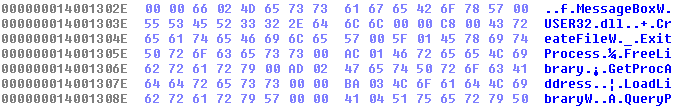
\includegraphics[width=1\linewidth]{Figures/windowsDemo64_Import_Name_Table}}
\caption{Import Name Table}
\label{fig:int}
\end{figure}

\begin{figure}[ht]
\fbox{\centering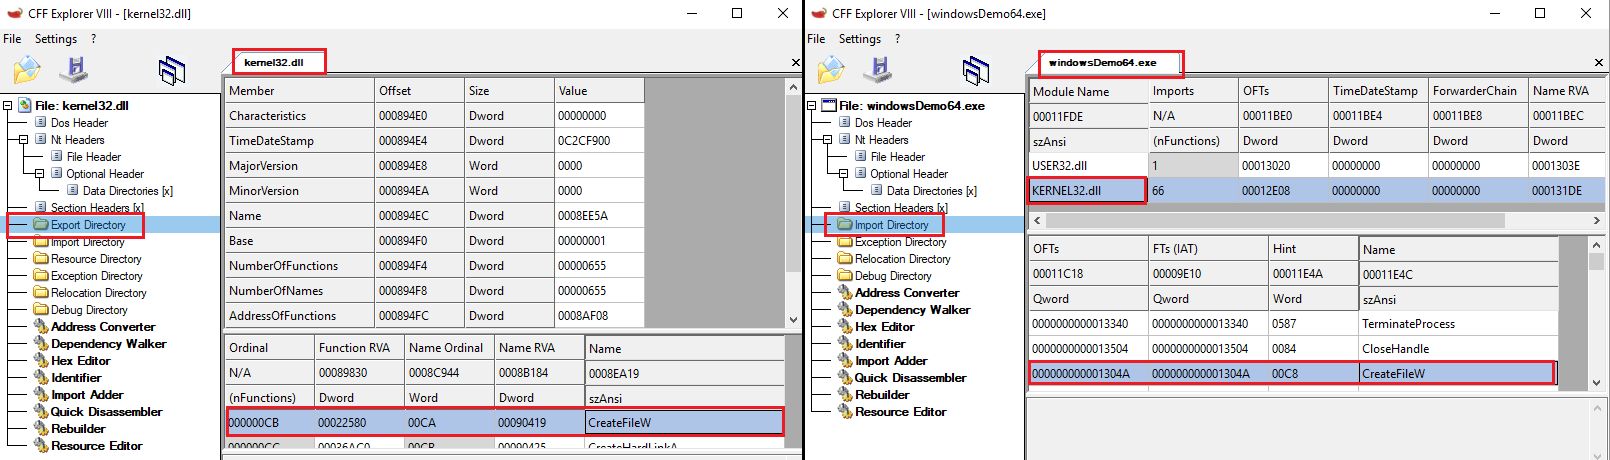
\includegraphics[width=1\linewidth]{Figures/Imports_and_Exports}}
\caption{Import Directory and Export Directory}
\label{fig:import_export}
\end{figure}

Let's step through this process using our example program and follow the flow of control for the \texttt{windowsDemo64.exe} call to \texttt{CreateFileW}. In Figure \ref{fig:import_export}, we show the compile time export directory of \texttt{kernel32.dll} on the left and the import directory of \texttt{windowsDemo64.exe} on the right. We used the CFF Explorer \cite{cffexplorer} tool to examine the PE32+ file structure. When the program is executed, the linker and loader can use these tables for resolution. Notice that the function RVA for \texttt{kernel32.dll}'s implementation is 0x22580. This means that the call cite for \texttt{CreateFileW} is located 140,672 bytes from the base address of \texttt{kernel32.dll}.

Examining the static disassembly of \texttt{windowsDemo64.exe}, we can locate the program's function call to \texttt{CreateFileW} at address 0x0140001098, as shown in Figure \ref{fig:windows64Demo_call_to_CreateFile}. Since this is a static analysis, it is important to keep in mind that the runtime addresses will change based on the operating system's choice for the image's base address. The object code for the function call is \texttt{FF15 729F0000}, where \texttt{FF15} are the opcodes for a \texttt{near call} and \texttt{729F0000} is the operand. The \texttt{near call} instruction operates by adding the operand to the value in the IP. Taking into account little-endian representation of the operand, we add \texttt{0x00009F72} to \texttt{0x0140001098} to find the entry in the import address table for \texttt{CreateFileW}. As shown in Figure \ref{fig:empty_IAT}, the pointer to \texttt{CreateFileW} is not filled in until linking and loading. 

\begin{figure}[ht]
\fbox{\centering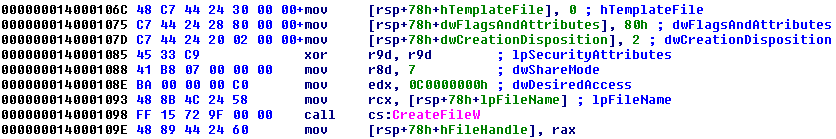
\includegraphics[width=1\linewidth]{Figures/windowsDemo64_call_to_CreateFile}}
\caption{User Program Call to CreateFile}
\label{fig:windows64Demo_call_to_CreateFile}
\end{figure}

\begin{figure}[ht]
\fbox{\centering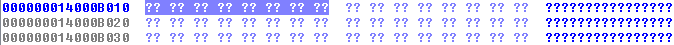
\includegraphics[width=1\linewidth]{Figures/Empty_IAT}}
\caption{Compile Time IAT}
\label{fig:empty_IAT}
\end{figure}

We attach the Windows Debugger (WinDbg) to \texttt{windowsDemo64.exe} to observe the process address space and the effects of linking and loading. Once the program was loaded, we observed the memory mappings as follows (some output truncated for clarity):\\\\
{\footnotesize{\texttt{0:002> lm\\
start \space\space\space\space\space\space\space\space\space\space\space\space end \space\space\space\space\space\space\space\space\space\space\space\space\space\space module name\\
00007ff7`1fe40000 00007ff7`1fe58000   windowsDemo64\\
00007ffb`7d0c0000 00007ffb`7d0d8000   myDLL64\\
00007ffb`81f70000 00007ffb`820a6000   wintypes\\
00007ffb`85e40000 00007ffb`85e60000   win32u\\
00007ffb`861b0000 00007ffb`86416000   KERNELBASE\\
00007ffb`872c0000 00007ffb`8736e000   KERNEL32\\
00007ffb`87370000 00007ffb`8740d000   msvcrt\\
00007ffb`87880000 00007ffb`87a0f000   USER32\\
00007ffb`899e0000 00007ffb`89bc0000   ntdll\\
}}}
\\From our previous static analysis, we know that the call to \texttt{CreateFileW} from \texttt{windowsDemo64.exe} is located at an offset of \texttt{0x1098} bytes from the base address. We add this offset to the base address observed above and disassemble the object code using WinDbg:\\\\
{\footnotesize{\texttt{
0:002> u 00007ff71fe41098 L1\\
windowsDemo64+0x1098:\\
00007ff7`1fe41098 ff15729f0000  call qword ptr [windowsDemo64+0xb010]
}}}
\\As expected, we observe the same object code as we saw in Figure \ref{fig:windows64Demo_call_to_CreateFile}. But now that the image has been linked and loaded, the IAT should no longer be empty as it was in Figure \ref{fig:empty_IAT}. We observe the contents of the pointer in the IAT in the same manner done previously, by adding the operand to the address of the next instruction.\\\\
{\footnotesize{\texttt{
0:002> dd 00007ff71fe4b010 L2\\
00007ff7`1fe4b010  872e2580 00007ffb
}}}
\\\\We see that the IAT entry for the call to \texttt{CreateFileW} is \texttt{00007FFB 872E2580}. This should point to the call site for \texttt{CreateFileW} inside of \texttt{kernel32.dll}. We observe the call site address and the disassembly of \texttt{kernel32.dll}'s implementation of \texttt{CreateFileW} as follows:\\\\
{\footnotesize{\texttt{
0:002> u kernel32!CreateFileW\\
KERNEL32!CreateFileW:\\
00007ffb`872e2580 ff2572240500  jmp qword ptr [KERNEL32!\_imp\_CreateFileW]
}}}
\\The address observed in the IAT is indeed a pointer to the call site for \texttt{CreateFileW} inside of \texttt{kernel32.dll}. We also observe that the call site is located at an offset of 0x22580 bytes from the base address of \texttt{kernel32.dll}, as expected from observations of DLL's export directory in Figure \ref{fig:import_export}. Interestingly, the code for this function is simply a jump into the DLL's own IAT. We observe the IAT entry as follows:\\\\
{\footnotesize{\texttt{
0:002> dd 00007ffb873349f8 L2\\
00007ffb`873349f8  861f1840 00007ffb
}}}
\\\\Disassembling the code at address \texttt{00007ffb 861f1840} shows that this is the call site into \texttt{kernelbase.dll}. Thus, \texttt{kernel32.dll} simply acts as an abstraction trampoline between the user program who calls the API function and the kernel's implementation.\\\\
{\footnotesize{\texttt{
0:002> u 00007ffb861f1840\\
KERNELBASE!CreateFileW:\\
00007ffb`861f1840 4883ec58  sub rsp,58h\\
00007ffb`861f1844 448b942488000000 mov     r10d,dword ptr [rsp+88h]
}}}
\\\\Only the first few lines of code are shown above, as it is a large function. We reverse engineered the function to observe that it is establishing a stack frame, allocating appropriate memory resources, and getting function parameters into position for it to eventually call \texttt{NtCreateFile}, which is imported from \texttt{ntdll.dll}. The \texttt{ntdll.dll} acts as the final abstraction barrier before the transition into kernel mode. The trap into kernel code is done via a \texttt{syscall} instruction. Before the system call, we see the value 0x55 being moved into the EAX register. Thus, the system call number for \texttt{NtCreateFile} is 85.\\\\
{\footnotesize{\texttt{
0:002> u ntdll!NtCreateFile\\
ntdll!NtCreateFile:\\
00007ffb`89a80910 4c8bd1 \space\space mov r10,rcx\\
00007ffb`89a80913 b855000000 \space mov eax,55h\\
00007ffb`89a80918 f604250803fe7f01 test byte ptr [SharedUserData+0x308 (00000000`7ffe0308)],1\\
00007ffb`89a80920 7503 \space\space\space jne ntdll!NtCreateFile+0x15 (00007ffb`89a80925)\\
00007ffb`89a80922 0f05 \space\space\space syscall\\
00007ffb`89a80924 c3 \space\space\space\space\space ret\\
00007ffb`89a80925 cd2e \space\space\space int 2Eh\\
00007ffb`89a80927 c3  \space\space\space\space\space ret
}}}\\\\
The traversal from user program through kernel32.dll to kernelbase.dll to ntdll.dll illustrates how the operating system puts up abstraction barriers between the user mode API call and the system call. Recall that kernel32.dll is simply a layer of redirection. This allows the underlying implementations to be updated and patched without disrupting the user program. For example, Windows is known to change system call numbers between versions and service packs. This also enforces compliance with the low level API. The kernelbase.dll acts a system call wrapper. It packages the user mode API call by setting up the registers and stack for the more complex system call. In Figure \ref{fig:API_vs_Syscall}, we compare the user mode API for \texttt{CreateFile} on the left, and the corresponding system call API for \texttt{NtCreateFile} on the right. 

\begin{figure}[ht]
\fbox{\centering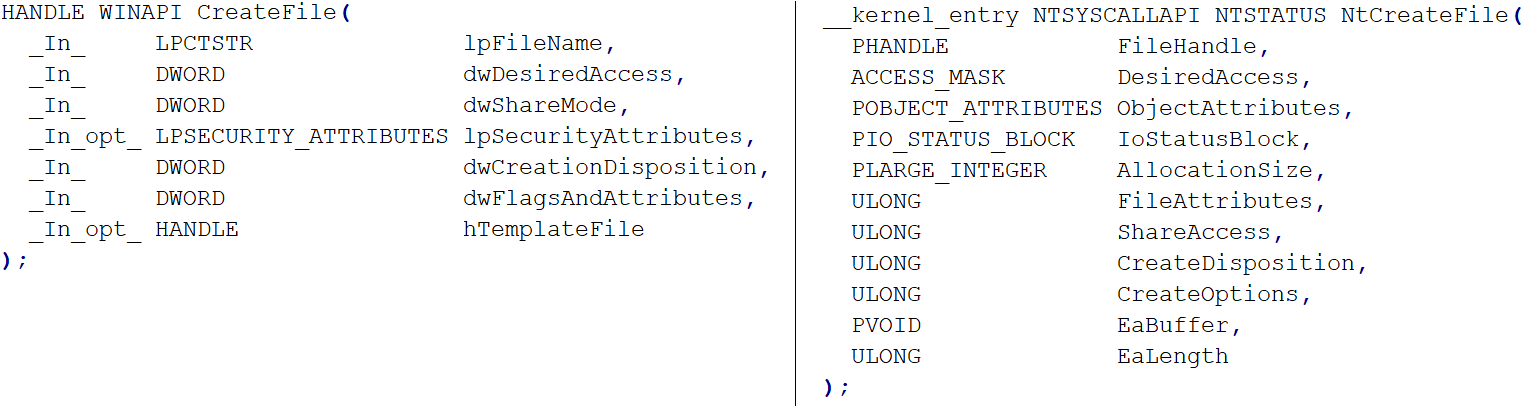
\includegraphics[width=1\linewidth]{Figures/CreateFile_API_and_System_Call}}
\caption{User Mode API vs System Call API}
\label{fig:API_vs_Syscall}
\end{figure}

When \texttt{ntdll.dll!NtCreateFile} is called, it issues the trap instruction \texttt{syscall} to switch into kernel mode. The system call number, 85 in our case, must be placed into EAX. This serves as an index into an array called \texttt{KeServiceDescriptorTable}. This is an array of integers that encodes the system call offset from EAX and the number of arguments that were passed onto the stack. When the \texttt{syscall} instruction is executed, it replaces the instruction pointer with the base address of the system call dispatcher. The CPU retrieves this address from a model specific register (MSR), which is IA32\_LSTAR MSR on IA64 architectures. During system initialization, Windows sets this register to point to the system call dispatcher. On Windows x64, we see that the primary system call dispatcher is \texttt{KiSystemCall64}. It is defined inside of \texttt{ntoskrnl.exe}, which is the kernel mode interface to the hardware abstraction layer. We generalize the flow of control over the abstraction barriers in Figure \ref{fig:abstraction}.

\begin{figure}[ht]
\centering\fbox{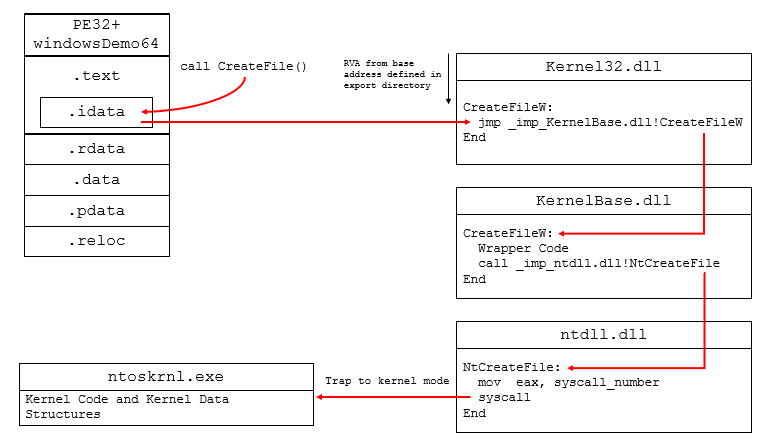
\includegraphics[width=1\linewidth]{Figures/User_Mode_to_Kernel_Mode}}
\caption{Windows Abstraction Barriers}
\label{fig:abstraction}
\end{figure}

Now that we have traversed a function call down into kernel code, we refer back to our program in Figure \ref{fig:windowsDemo64.c} to discuss delay loading and explicit runtime linking. As previously discussed, programs that import functions from dynamically linked libraries normally reserve a section in the compiled binary for the linker to fill in the pointers. With delay loading, there is no compile time reference to the external library. In our test program, we tested the effects of delay loading by importing a simple custom DLL, \texttt{myDLL64}, at runtime. Notice that there is no entry for \texttt{myDLL64} in the program's import directory in Figure \ref{fig:import_export}. The Win32 \texttt{LoadLibrary} is used to load an image into the process's address space. Then explicit runtime linking is achieved by calling \texttt{GetProcAddress} to retrieve a pointer to an imported function from the newly loaded library. Figure \ref{fig:delayloading} shows our program importing a function called \texttt{Message} from \texttt{myDLL64}. The name of the DLL is the argument to \texttt{LoadLibrary}, which returns a handle that is used as an argument, along with the name of the desired function, to \texttt{GetProcAddress}

\begin{figure}[ht]
\centering\fbox{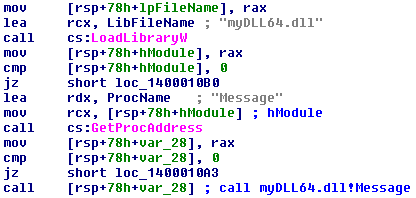
\includegraphics[width=.5\linewidth]{Figures/delayLoading}}
\caption{Delay Loading and Explicit Runtime Linking}
\label{fig:delayloading}
\end{figure}

Tracing through the program with a debugger, we did not observe the mapping of the DLL into the process address space until \texttt{LoadLibrary} was called. Figure \ref{fig:memorymap} shows the memory mappings of the DLL in the process address space.

\begin{figure}[ht]
\centering\fbox{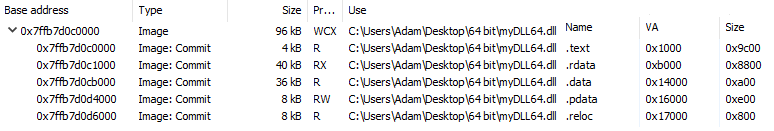
\includegraphics[width=.5\linewidth]{Figures/Memory_Mapped_DLL}}
\caption{Memory Mapped DLL}
\label{fig:memorymap}
\end{figure}

We present a discussion on delay loading and explicit runtime linking because of its relevance in finding code similarities. A popular way to find variants of the same malware is to calculate the hash of the import directory, called the ImpHash \cite{imphash} \cite{choi2015malware}. Intuitively, this similarity technique should be effective because it is opcode agnostic and can therefore overcome compiler diversification. However, the ImpHash does not consider delay loading, embedded executable images hidden elsewhere in the PE32 that may contain an import directory, or obfuscated API calls \cite{suenaga2009museum} \cite{srivastava2008system} \cite{o2011obfuscation}. Further, we argue that delay loading and other import directory hiding techniques can thwart static control flow graph (CFG) analysis based on API extraction \cite{alazab2010towards}. We propose improvements in Section 6.

\subsection{Linux Control Flow}

In this section we briefly discuss control flow in Linux systems. For brevity, our treatment on Linux will not be as in depth as our treatment of Windows. A simple C program was written to demonstrate how the Linux Executable Linkable File (ELF) file structure is constructed for linking to external libraries. The disassembly of main for our simple program is shown in Figure \ref{fig:hellomain}. It simply calls \texttt{printf} to print a hard coded string "Hello" and the command-line argument.

\begin{figure}[ht]
\centering\fbox{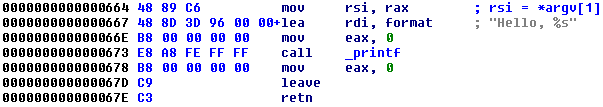
\includegraphics[width=.5\linewidth]{Figures/hello_main}}
\caption{Disassembly of Main of Compiled Hello Program}
\label{fig:hellomain}
\end{figure}

The call to \texttt{printf} points to an entry in the ELF's procedure linkage table (PLT). The PLT contains a small stub entry for the external function. As shown in Figure \ref{fig:plt}, the PLT entry for \texttt{printf} is simply a layer of indirection implemented as a jump into the global offset table (GOT). The GOT, shown in Figure \ref{fig:got}, will be filled in with the address of the function by the runtime linker. 


\begin{figure}[ht]
\centering\fbox{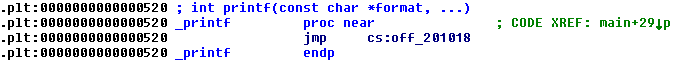
\includegraphics[width=.5\linewidth]{Figures/plt_printf}}
\caption{Program Linkage Table (PLT) Entry for printf}
\label{fig:plt}
\end{figure}

\begin{figure}[ht]
\centering\fbox{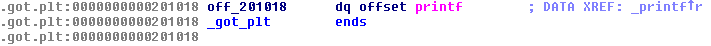
\includegraphics[width=.5\linewidth]{Figures/got_printf}}
\caption{Global Offset Table (GOT)}
\label{fig:got}
\end{figure}

Similar to how the linker resolves exports and imports via RVAs in Windows, the runtime linker will fill in the GOT when the program is loaded into memory. The purpose of the indirection provided by the PLT is to enable lazy on-demand binding. The runtime linker will fill in the addresses to the functions in shared object files (.so) when the program calls the first function from that library. When the library procedure is called, it will wrap the user mode function into the appropriate ABI for the system call. The wrapper function will also place the appropriate system call from the syscall table into the RAX register before the syscall instruction is called. As already mentioned, the syscall instruction replaces the instruction pointer with the address of the system call handler located in the LSTAR MSR register.

Understanding program control flow and all of the abstraction barriers in operating systems is a necessary prerequisite for further research in code randomization and control flow integrity. Since modern exploits rely heavily on memory disclosure \cite{szekeres2013sok}, we must understand how the readable memory pages contain valuable information that can be useful for an attacker to craft a runtime code reuse and control flow hijacking attack. Readable information such as function pointers, relative offsets, and return addresses from the stack can glean information about the code layout, enabling the construction of ROP chains that are capable of bypassing modern defenses. Code randomization, control flow integrity, and additional operating system memory protections are several proposed solutions to make this process more challenging.

\section{Threat Model}
\label{S:3}

For our discussion, we generalize the attack pattern into two phases. The first phase is software exploitation. This is where the attacker exploits a vulnerability in the software. The attacker uses the vulnerability to achieve malicious effects. These actions on the target are the second phase of the attack. During this second phase, the attack manipulates the program control flow of the target process. 

Memory corruption and memory disclosure vulnerabilities in conjunction with overflow vulnerabilities offer attackers a mechanism to exploit the software, achieving the first phase of the exploitation process. Format string vulnerabilities, dangling pointers, unchecked heap and buffer boundaries are some of the more popular exploitation techniques. \cite{szekeres2013sok} provides a systemization and overview of these memory vulnerabilities.

Once the attacker identifies and exploits the initial memory vulnerability, they can craft a payload to leverage this injection vector to achieve effects, which is phase two. During this phase, the attacker needs to manipulate the control flow of the victim process in order to execute the attacker's desired code. Traditional stack based shellcode injection has been rendered ineffective thanks to Data Execution Prevention (DEP), which enforces write XOR execute privilege policy on memory mapped code and data pages. Thus, attackers have adapted to use code reuse attacks to achieve effects on target. Code reuse attacks modify the flow of control by executing code already mapped into the process's address space \cite{shacham2007geometry}. This reduces the need to rely on injected code via stack smashing \cite{aleph1996smashing}.

Return oriented programming (ROP) attacks, or the more general code reuse attack, makes use of existing code sequences called gadgets in order to manipulate control flow \cite{shacham2007geometry}. From our reverse engineering exercise on control flow and program execution in Section 2, we observe that the overall attack surface for user programs is much larger than just the programmer defined instructions. Libraries, system call wrappers, and operating system abstraction barriers offer a large attack surface to manipulate control flow. ROP attacks focus on finding small gadgets of code that end in a \texttt{ret} instruction to achieve arbitrary code execution in the address space of the victim process. The instruction pointer is heavily controlled by \texttt{ret}, which pops a function's return address off the stack and places it into the instruction pointer. Thus, attackers can overwrite the return value on the stack by taking advantage of one of the many stage one vulnerabilities discussed in \cite{szekeres2013sok}. Then the attack invokes a \texttt{ret} to force the instruction pointer to execute the desired code. \cite{shacham2007geometry} demonstrates that arbitrary code execution can be achieved without introducing any new code by finding gadgets. These gadgets are short sequences of opcodes that can be used to load function parameters into registers, store values in desired registers, and then end in a ret in order to control execution. The gadget sequence of \texttt{pop \%reg, ret} can be especially helpful for loading desired parameters before invoking a function or a system call.

\cite{shacham2007geometry} further shows how unintended code sequences can introduce a Turing complete platform for attackers to find gadgets. For example, consider Figure \ref{fig:Gadget}. The compiler generated code who intended to start execution via a function pointer at instruction 0x00401012. The disassembly shows this as a mov and a jmp instruction. Suppose the attacker, through memory corruption, indexed the function pointer by two. Now we see a new sequence of instructions that end in a ret. The attacker can chain these types of gadgets together via ROP-chaining in order to achieve arbitrary code execution.

\begin{figure}[ht]
\centering\fbox{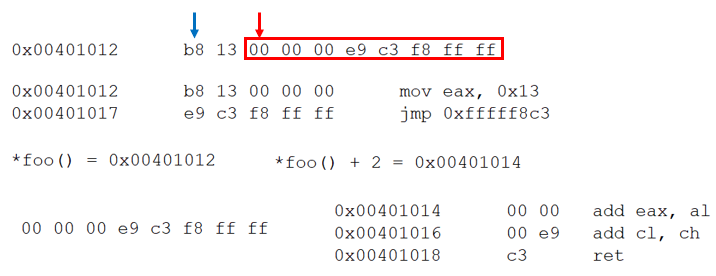
\includegraphics[width=.5\linewidth]{Figures/Gadget}}
\caption{Unintended Code Sequence}
\label{fig:Gadget}
\end{figure}

Similar types of control flow attacks have been introduced in addition to ROP. Jump oriented attacks try to manipulate jump instruction operands via indirect register addressing \cite{bletsch2011jump}. This technique removes the reliance on \texttt{ret} instructions. \cite{payer2013string} propose string oriented programming (SOP), which relies on format string vulnerabilities to overwrite control data on the stack as a code reuse capability. \cite{snow2013just} offer a technique called just-in-time ROP attacks (JIT-ROP). These attacks can overcome code randomization by finding gadgets at runtime. Advances in defenses, discussed in the next section, have tried to mitigate many forms of code reuse attacks that rely on memory leakage. However, offensive research responds with more comprehensive attacks. For example, \cite{rudd2017address} propose address oblivious code reuse attacks (AOCR). In AOCR, attackers perform offline analysis of programs that have been protected with code randomization and reduced memory disclosure. This attack uses inference to identify the code layout, such as function pointers, function calling patterns, and relative locations. They also introduce malicious thread blocking, which is a technique that forces a thread to block while waiting on a mutex. This blocking affords the attackers time to develop JIT-ROP attacks against a diversified and protected application. \cite{schuster2015counterfeit} demonstrate a code reuse attack on C++ applications called counterfeit object oriented programming (COOP). This attack vector exploits the predictability of vtables (virtual function call dispatch tables) in compiled binaries. They demonstrated how memory leakage can disclose function pointers in vtables, and control flow can be manipulated to invoke vtable functions, agnostic of object inheritance.

In the next section, we survey some of the influential work in defending against code reuse and memory disclosure attacks.

\section{Survey of Defenses}
\label{S:4}

Attempts to thwart code reuse attacks as a result of memory disclosure mostly come in three flavors: randomization, control flow integrity, and software booby traps. In this section, we survey the influential research in these areas. Since we are also interested in addressing the need to classify diversified malware, We also present a discussion on software similarity testing.

\subsection{Compiler Defenses}

Compiler-generated code randomizations and diversification aims to create uncertainty in the attack surface to defeat pre-configured ROP and code reuse attacks. Uncertainty is created by generating a unique, yet semantically equivalent, compiled binary for each compilation. The randomization can be introduced in the optimization phase of the compiler toolchain, as shown in Figure \ref{fig:compiler}. Larsen et. al. \cite{larsen2014sokautomated} provide a systemization for compiler-generated software diversification. They also provide a more in-depth discussion in \cite{larsen2015automated}. We summarize their discussion below. 

\begin{figure}[ht]
\centering\fbox{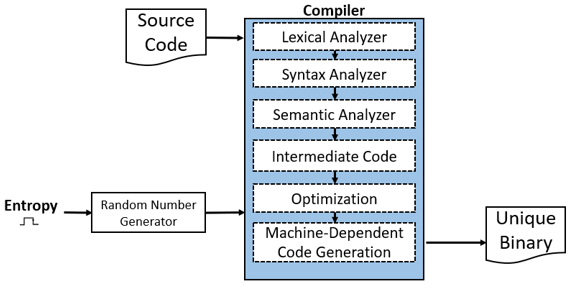
\includegraphics[width=.5\linewidth]{Figures/compiler}}
\caption{Compiler Generated Randomization}
\label{fig:compiler}
\end{figure}

One of the simplest techniques that the compiler can utilize to generate diversity is randomized NOP insertion. The NOP instruction (opcode 0x90 in x86), simply consumes a clock cycle, and does not impact any of the flags on the processor status register. It is therefore an intuitive candidate to randomize the binary without impacting semantics. Randomized NOP insertion creates different offsets and relative addresses for each instance of the compiled application. It also has a large effect on the relocation tables (.reloc section discussed in Section 2). Since each application will have its code and return addresses at different locations, precompiled ROP attacks will need to be adjusted for each individual instance of the binary, thereby reducing the scalability of the attack.

Instruction substitution is a compiler technique where different instructions are generated. Observing that the x86\_64 instruction set is a variable length architecture, instruction level variation will impact the offsets and relocations. To observe the variation in object code with semantically equivalent instructions, we generated some samples using the MASM assembler in Figure \ref{fig:instructions}. Observe that each instruction performs the same task, but with large deviations in object code. Similarly, instruction permutation randomizes the order in which the instructions are generated. This is of coarse dependent on pipelining and register dependencies, but can it can introduce variance in the compiled object code size and thus randomize ROP gadget locations, and available ROP gadget sequences.

\begin{figure}[ht]
\centering\fbox{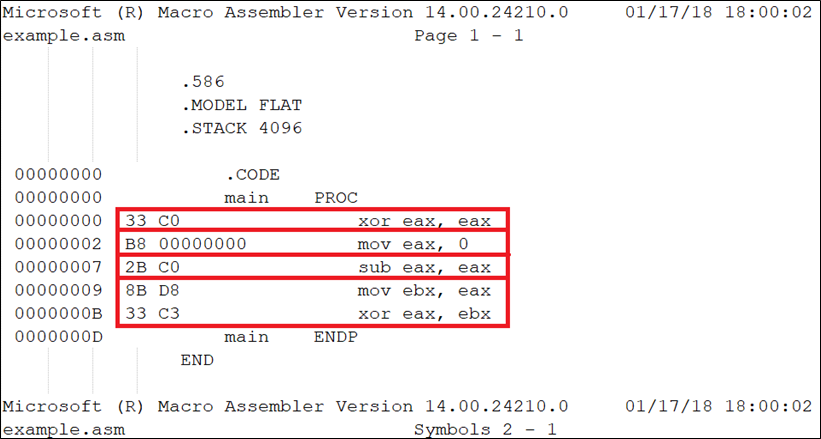
\includegraphics[width=.5\linewidth]{Figures/instructions}}
\caption{Instruction-Level Variations}
\label{fig:instructions}
\end{figure}

Function shuffling is another compiler approach in which the nature of function calls are randomized. This includes function calling notations, introducing polymorphic function arguments, and randomizing the function calling order. This can be extended to randomize the order of library API calls.

Another compiler technique was introduced in Readactor \cite{crane2015readactor}. They observed that ROP and JIT-ROP \cite{snow2013just} attacks require memory disclosure from code pointers. This includes function pointers, return addresses, and dynamic linker structures (such as the PLT and GOT in ELF binaries). Thus, Readactor implemented an LLVM modification that creates code trampolines to prevent memory disclosure. All pointers, addresses, and control flow information are replaced with a jump instruction into a randomized execute-only trampoline section. The trampoline then simply redirects control to the desired call site. They implemented the execute-only permissions via a thin hyperviser that uses Intel Extended Page Tables (EPT). Therefore, the true layout of the code cannot be determined at runtime due to the added layer of indirection. Readactor also implemented code randomization techniques, such as function reordering and randomized NOP insertion.

At the same conference that Readactor was presented, the counterfiet object oriented programming (COOP) attack \cite{schuster2015counterfeit} was presented, which exploits the disclosure of virtual function pointer tables (vtables) in C++ applications. The authors of Readactor responded with Readactor++ \cite{crane2015s}. Readactor++ randomizes the vtable layer at each pass of the compiler to defeat COOP attacks. 

In 2017, Rudd et al. \cite{rudd2017address} introduced address-oblivious code reuse (AOCR) attacks. They launched code reuse attacks against Readactor protected applications by profiling. They conduct offline analysis to profile the target application's control flow in order to infer code layout and behavior. From this, they successfully launched code reuse attacks without relying on memory disclosure. They further utilized a novel technique called malicious thread blocking (MTB), where they obtain a mutex to block a thread's execution. This blocking affords the attackers time to collect information and perform disassembly of code pages to further target the attack. To the best of our knowledge, their is no existing literature that claims to defeat AOCR attacks.

The biggest limitation of compiler-generated diversification is the need for source code access and compiler modifications. This can pose a problem for pre-compiled libraries that a protected program may map into its address space. However, operating system diversification may be able to augment compiler-generated application randomization to assist with defeating software attacks. 

\subsection{Operating System Interface Diversification}

In \cite{Rauti14}, the authors propose a system call diversification technique that randomizes the system call numbers in the Linux syscall table. The intent is to protect computers from malicious code that is executed as its own process or as part of another process. It appears that they diversify once after compilation, but before execution, then perform a linear sweep on all compiled binaries to search for \texttt{syscall} instructions and replace the argument with the new syscall number. I suspect that this approach leaves the system vulnerable to code reuse attacks. Another thing the authors do not consider is cloning, which is when a fork() creates a duplicate mapping, which can maybe leak memory mappings to system calls. I also suspect this approach is vulnerable to memory leaks. We need to investigate the effects on the GOT and PLT with this approach. The authors also acknowledge the difficulty in accurately updating the register arguments for the syscall numbers during the linear sweep due to gaps in code. It will also be interesting to see if this approach can be duplicated in Windows by hooking \texttt{ntdll.dll}.

\cite{abrath2015obfuscating} proposes two techniques to diversify the interface between user programs and the kernel by obfuscating Windows DLLs. The first method removes the IAT from the compiled binary and introduces a custom loader to load APIs from a hash table. They use LoadLibrary(), which is resolved by traversing the PEB, similar to how shellcode achieves position independence. They implement this via a link-time rewriter in the Diablo framework. The second method is to statically link the DLLs into the binary and apply diversification. They lift the binary into Diablo's IR, obfuscate the IR, then further randomize code placement. This increases the size of the binary, and removes portability across different Windows versions. They do not consider delay loading, runtime explicit linking, nor linking by ordinal.

\cite{jiang2007randsys} proposes comprehensive operating system diversification through instruction set randomization, ABI obfuscation, and low-level memory randomization. This technique introduces a significant performance overhead and requires hardware modifications, making widespread deployment unfeasible. \cite{li2010defeating} also propose kernel code modifications to create ret-less kernels to defeat ROP rootkits. Without return instructions, rootkits cannot exploit the inherit memory leakage of return addresses on the stack. However, we are inclined to suspect that this technique is not comprehensive, still allowing jump oriented attacks, function reuse attacks, and other variants of code reuse that do not rely on the return instruction. \cite{gionta2016preventing} later proposed fine grained code randomization in kernel space to defend against kernel code reuse attacks. However, it is unknown if this technique can defeat AOCR attacks.

\cite{criswell2014kcofi} offer a control flow integrity (CFI) approach to protecting kernels. This technique requires compiler support and access to kernel source code. They introduce CFI checks in kernel routines to make sure that system calls, when dispatched, execute the predefined control path. Deviation will result in a raised exception which must be handled by the operating system. kGuard \cite{kemerlis2012kguard} is another kernel protection mechanism that combines kernel code randomization with control flow assertions (CFAs). Similar to stack canaries, CFAs are implemented at indirect jumps and function calls to ensure that privileged kernel execution remains within the boundaries of kernel space. This prevents the return-to-user attack, which is a privilege escalation attack that hijacks the control flow of kernel code to jump outside of the abstraction barrier during privileged kernel code execution.

More recently, \cite{pomonis2017kr} proposed a read xor execute policy (similar to \cite{brookes2016exoshim}) in kernel code combined with kernel code diversification. The R xor X policy reduces memory disclosure, since code pages are no longer readable. They also enforce a return address protection mechanism through xor encoding. The R xor X policy is enforced in kernel space through fine grained segmentation of kernel module files (.ko). The .text and .data segments of the .ko modules are segmented into different memory mapped regions with different permissions. The CPU is still able to fetch instructions from read-only memory regions. Kernel code memory layout can still be inferred through side channel attacks, such as timing analysis and paging system channels as indicated in \cite{gens2017lazarus}. Thus, they proposed a more fine-grained KASLR mechanism called Lazarus, which introduces randomization into the paging algorithms in the kernel.

\subsection{Runtime Randomization}

Runtime randomization involves memory and code layout randomization at runtime. Davi et al. \cite{davi2015isomeron} propose a defense called Isomeron that tolerates code disclosure by randomizing function return addresses on the stack at runtime. The authors claim that the Isomeron thwarts JIT-ROP attacks, because it is not known until the function is called what the return address will be on the stack. \cite{friedman2015chronomorphic} propose rewriting binaries into chronomorphic applications who randomize their in-memory instructions and program layout at runtime. \cite{hawkins2017mixr} similarly proposes runtime diversity, but they provide a highly configurable diversification platform. The defender can configure randomization parameters, such as memory ranges and code blocks.All observed runtime randomization techniques incur heavy performance hits, making them undesirable as they currently stand.

\subsection{Software Deception}

In 2013, Crane et al. \cite{crane2013booby} first pontificated over the possibility of booby trapping software. This paper was conceptual, discussing the potential benefits of leaving tripwires in software to alert defenders of an attack. Booby-trapped software can include leaving attractive code gadgets throughout the software that serve no other purpose than to throw an exception when that execution path is invoked. Deceptive vtables, function pointers, and control flow information can be incorporated to entice attackers to trigger a tripwire, such as a special purpose exception handler. Araujo et al. \cite{araujo2014patches} propose software honey-patches to misdirect attackers. They further develop this concept to deceive attackers into thinking they were successful in \cite{araujo2015compiler}. They modify the LLVM compiler toolchain to perform a taint analysis to see which data can be influenced from external sources (i.e. an attacker), and use this information flow to deceive attackers if malicious input is detected. A very similar concept was more recently discussed in Avery et al's 2017 paper on Ghost Patches \cite{avery2017ghost}. They propose a deceptive maneuver that involves inserting tripwires into software patches. In section 6, we consider leveraging deception to invoke runtime rerandomization.

\subsection{Similarity Detection}

In this section, we review the influential work in malware similarity testing. In section 6, we further consider the implications of malware introducing diversification to defeat known similarity techniques. \cite{payer2014embracing} first introduced this concern, and further demonstrated that common similarity detection techniques can be defeated with code and data diversification in \cite{payer2014similarity}.

Recently, Pagani et al \cite{pagani2018beyond} analyzed the effectiveness of various fuzzy hashing techniques to classify malware of similar variants. There study included a discussion on identifying the same source from different compiler flags, but they did not consider explicit compiler generated diversification as discussed previously in section 4.1. Their study was able to shine some light on why certain similarity algorithms work better than others in various situations. We summarize their findings as follows:

\begin{itemize}
  \item ssdeep only works for files in similar size and with very few modifications.
  \item tlsh is preferable when dealing with source code changes.
  \item sdhash is preferable when dealing with compiler toolchain changes.
\end{itemize}

They discuss how very small changes can throw off similarity detection due to offsets and relocations changing. As discussed earlier with compiler diversity, these changes are desired for randomizing an attack surface. The findings are interesting, but we feel there is more work to be done in this field. For example, this study should consider malware diversity as discussed in \cite{payer2014embracing}. Further, the authors did not consider 32-bit versus 64-bit files. The difference in compilation and object code between 32-bit and 64-bit binaries is vast. During our reverse engineering exercise in Section 2, we observed that relocations are not used as heavily as in 32-bit binaries. That is because x64 introduced the ability to reference call sites and jump destinations as offsets from the instruction pointer. This alleviates a need for the linker to resolve the destination operands from the relocation tables. Further, the function calling conventions vary drastically between 32 and 64 bit variants. We compiled and analyzed the 64-bit and 32-bit variant of the same program from Section 2 using the same compiler. As shown in Figure \ref{fig:32-64}, we observe drastic changes in the object code. Notice the change in calling convention and the lack of using relocations in the 64-bit variant. 

\begin{figure}[ht]
\centering\fbox{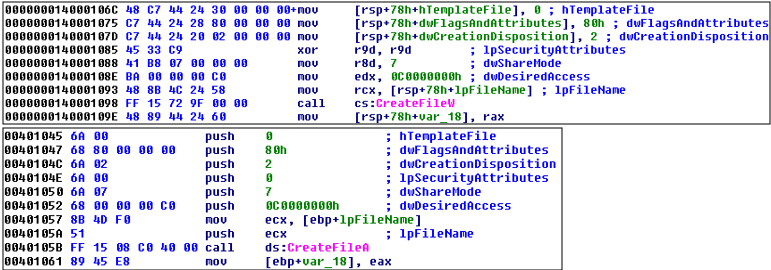
\includegraphics[width=.5\linewidth]{Figures/32-64}}
\caption{32-bit versus 64-bit}
\label{fig:32-64}
\end{figure}

Upchurch and Zhou \cite{upchurch2016malware} recently proposed a technique of Malware Provenance that abstracts away the opcode operands and only observes the first opcode in a sliding window fashion to find similar code blocks. Although this technique is fast and effective for recall and identifying code reuse, we argue it is not robust against a diversified sample. For example, consider the instruction substitutions in Figure \ref{fig:instructions}. These instructions clearly have different opcodes, and would not be classified as identical even though they are semantically equivalent. Thus, we opine that the approach in \cite{upchurch2016malware} should be tested against compiler variations and be modified to an abstraction of the actual opcodes.

David et al. \cite{david2017similarity} proposed in their 2017 PLDI paper a technique to find similar code patterns using binary lifting and reoptimization. They lifted compiled binaries into the LLVM intermediate representation to find similar code fragments for vulnerability searching. They do not consider malware similarity under a diversified corpus, but we opine that their approach can be extended to normalize compiled binaries to see if diversified malware can be successfully classified as similar.

There are also a number of call graph techniques to detect similarity \cite{jang2014mal} \cite {singh2017malware} \cite{hassen2017scalable}. However, it is unknown if these techniques are robust against function level diversification. Further, call graphs can vary based on branching, and fine-grained call graphs often require dynamic analysis, which is computationally expensive compared to static analysis.

\section{Key Papers}

In this section, we condense the literature survey into twelve influential papers on the topics of code diversification, deception, and code similarity.

\subsection{
\cite{shacham2007geometry} Shacham, Hovav. "The geometry of innocent flesh on the bone: Return-into-libc without function calls (on the x86)." In Proceedings of the 14th ACM conference on Computer and communications security, pp. 552-561. ACM, 2007.
}

Summary: This paper is one of the original influential works in code reuse attacks. They document the discovery of code gadgets in x86 binaries through static analysis techniques. They demonstrate how to deploy return-into-libc attacks through control flow redirection. They make use of readable code pages and the readable return addresses on the stack to redirect control into the GNU C library, enabling arbitrary C library function calls.

Assessment: We chose this paper as an influential work because it documents in technical depth the mechanics of the return-into-libc attack. We observed that this paper was cited in almost every ROP related paper we analyzed. Further, it influenced a lot of research on more advanced code reuse attacks, including jump oriented programming \cite{bletsch2011jump}, JIT-ROP \cite{snow2013just}, AOCR \cite{rudd2017address}, and COOP \cite{schuster2015counterfeit}.

Relation to Research: This paper can influence our research since it provides the foundational mechanics for understanding how control flow can be redirected via indirect memory disclosure. After reading this paper, it is clear how the readable memory pages (such as the stack) and the predictable code layout can offer attackers the opportunity to take advantage of the x86 calling convention and stack layout to invoke arbitrary library functions.

\subsection{
\cite{larsen2015automated}, Per, Stefan Brunthaler, Lucas Davi, Ahmad-Reza Sadeghi, and Michael Franz. "Automated software diversity." Synthesis Lectures on Information Security, Privacy, \& Trust 10, no. 2 (2015): 1-88.
}

Summary: This paper provides a detailed overview on  the state of the art on compiler-generated code randomization and diversification. Authored by the leading researchers in the field, most of the work they summarize and analyze is their previous work. Therefore, this paper nicely condenses a large body of code diversification papers into a convenient reference. A more in-depth discussion on the mechanics is provided in Section 4.1.

Assessment: The authors propose compiler-generated diversification and randomization to defeat the code reuse attacks. They argue that an unpredictable and dynamic code layout can make predicting code gadgets utilizing return addresses unreliable.

Relation to Research: One of our research tasks is to detect similar applications and similar code fragments that can overcome diversification. Therefore, an understanding of code randomization techniques is essential. This paper nicely summarizes common compiler tactics without sacrificing technical depth.


\subsection{
\cite{crane2015readactor} Crane, Stephen, Christopher Liebchen, Andrei Homescu, Lucas Davi, Per Larsen, Ahmad-Reza Sadeghi, Stefan Brunthaler, and Michael Franz. "Readactor: Practical code randomization resilient to memory disclosure." In Security and Privacy (SP), 2015 IEEE Symposium on, pp. 763-780. IEEE, 2015.
}

Summary: Readactor is the first compiler technique to drastically reduce memory disclosure through layers of indirection. They replace all function call sites, return addresses, and linker information with jumps to a read-only trampoline section that is randomized. The trampoline simply contains jumps into the actual code sections, that are also protected with read-only permissions.

Assessment: This paper combines compiler-generated code randomization with operating system support of enforcing read-only code pages to protect applications against code reuse by hiding the true layout of an application. It is also interesting to note that a Readacted ELF application does not contain a GOT nor a PLT (see Section 2.2). The compiler instead produces pointers to protected trampolines, which is where the linker will insert pointer information. One thing that is not discussed in the paper in much depth is how the runtime linker can write to a read-only memory page. We suspect that the permissions are not enforced until after the linker and loader have completed their pass, which leaves a small period of time where an attacker can infer code layout. It was shown in \cite{rudd2017address} that Readacted applications are vulnerable to AOCR attacks.

Relation to Research: This paper is the first to propose additional layers of indirection to protect applications from memory disclosure. Since this approach requires access to source code and compiler modifications, we consider the possibility of leveraging indirection elsewhere. Relocation tables and import and export tables are potential candidates for additional redirection for both defensive and offensive purposes. As a defender, it can prevent the disclosure of libc and library API locations. As an offender, it can potentially render import related similarity testing \cite{imphash} ineffective. It is also interesting to point out that we observed layers of indirection in operating system abstraction barriers in Section 2.

\subsection{
\cite{rudd2017address} Rudd, Robert, Richard Skowyra, David Bigelow, Veer Dedhia, Thomas Hobson, Stephen Crane, Christopher Liebchen et al. "Address-Oblivious Code Reuse: On the Effectiveness of Leakage Resilient Diversity." In Proceedings of the Network and Distributed System Security Symposium (NDSS’17). 2017.
}

Summary: This paper demonstrates the real challenge with preventing all forms of memory disclosure. They demonstrate attacks on Readacted protected applications that bypass code randomization and memory leakage resilience. They perform offline code analysis through reverse engineering and function profiling to identify call patterns. Then, they introduce malicious blocking, which forces a victim thread to enter a blocked state. The combination of inference analysis and time leveraged while the thread is blocked provided the attack vector with enough time to create a reliable JIT-ROP payload.

Assessment: This paper demonstrated a weakness in Readactor and code randomization and code layout hiding in general. Readactor, which is an otherwise promising tactic, cannot completely hide the semantics of a program. We also found the malicious thread blocking (MTB) technique interesting because it affords the attackers time to infer the target address space. To our knowledge, there is no literature that argues a defense against this class of attacks.

Relation to Research: This paper proves that memory disclosure resilience is hard. Since this is the latest in offensive code reuse research, resilience to the AOCR attack should be considered. 

\subsection{
\cite{Rauti14} Rauti, Sampsa, Samuel Laurén, Shohreh Hosseinzadeh, Jari-Matti Mäkelä, Sami Hyrynsalmi, and Ville Leppänen. "Diversification of system calls in Linux binaries." In International Conference on Trusted Systems, pp. 15-35. Springer, Cham, 2014.
}

Summary: The authors explore randomizing the system call numbering scheme in Linux operating systems to render the execution environment incompatible. They simply randomly rearrange the system call number in the system call table. Then they perform a linear sweep on all of the binaries that directly invoke the system call and make the appropriate swap. This also requires adjusting parameters and register assignments.

Assessment: This will surely render injected shellcode incompatible with the operating system, since shellcode contains direct invocations of the syscall instruction. However, we don't believe this approach will protect against code reuse attacks. We also do not believe this approach will scale well to Windows platforms, since the Windows system call numbering convention vary between versions, and attacker's typically invoke the abstraction of kernel32.dll or the system call wrapper in ntdll.dll instead of the actual system call. 

Relation to Research: Randomizing the underlying operating system components is an alternative to randomizing the application. This particular system call randomization approach, although likely ineffective against ROP attacks, has potential to be modified to incorporate runtime diversification. This concept can be extended to randomize interrupt handling routines (interrupt descriptor table, IDT), exception handlers, and other operating system routines. Further, it may be worthwhile to consider system call authorizations. For example, we call look into making sure system calls are only invoked in accordance with an application's control flow integrity.

\subsection{
\cite{crane2015s} Crane, Stephen, Stijn Volckaert, Felix Schuster, Christopher Liebchen, Per Larsen, Lucas Davi, Ahmad-Reza Sadeghi, Thorsten Holz, Bjorn De Sutter, and Michael Franz. "It's a TRaP: Table randomization and protection against function-reuse attacks." In Proceedings of the 22nd ACM SIGSAC Conference on Computer and Communications Security, pp. 243-255. ACM, 2015.
}

Summary: This paper was written in response to COOP attacks \cite{schuster2015counterfeit}, which targeted vtables in C++ applications. This paper extends upon Readactor \cite{crane2015readactor} to create Readactor++, which includes vtable randomization and trampoline code for virtual functions.

Assessment: It is interesting to observe the evolution of this line of research, from \cite{crane2015readactor}, to \cite{schuster2015counterfeit}, to \cite{crane2015s}. This is an example of how fast this research is moving to develop both new offensive and defensive tactics. This paper solves the problem of memory disclosure provided by vtables by introducing more randomization in the vtable layout and hiding the true call sites for the functions through indirection.

Relation to Research: Readactor++ seems to be the most comprehensive code diversification and layout randomization scheme we have observed in our literature survey. This technique was proven vulnerable to AOCR attacks \cite{rudd2017address}. Thus, we can consider the possibility of introducing booby trapped virtual functions in the vtables to alert the defenders of an active code reuse attack. We can use the indirection and pointer hiding techniques presented in this paper to hide the exception handling routines that are thrown when a booby trap is triggered.

\subsection{
\cite{snow2013just} Snow, Kevin Z., Fabian Monrose, Lucas Davi, Alexandra Dmitrienko, Christopher Liebchen, and Ahmad-Reza Sadeghi. "Just-in-time code reuse: On the effectiveness of fine-grained address space layout randomization." In Security and Privacy (SP), 2013 IEEE Symposium on, pp. 574-588. IEEE, 2013.
}

Summary: JIT-ROP was a breakthrough in offensive research. With JIT-ROP, attacks can bypass code randomization by building ROP gadgets on the fly. This changed the game drastically, and inspired ROP defenses to focus more on memory disclosure instead of layout randomization \cite{crane2015readactor} \cite{crane2015s}.

Assessment: This approach analyzed the code layout at runtime to detect gadgets. One interesting thing we observed was the author's use of LoadLibrary to gain arbitrary code execution. We assess that loading external libraries could be detected with a coarse grained control flow integrity. 

Relation to Research: In Section 6.2, we will discuss the possibility of examining memory mappings for control flow integrity. We believe this can deter JIT-ROP attacks proposed in this paper, since they rely on mapping the desired libraries to the target address space in order to achieve code execution.

\subsection{
\cite{payer2014embracing} Payer, Mathias. "Embracing the new threat: Towards automatically self-diversifying malware." In The Symposium on Security for Asia Network. 2014.
}

Summary: This paper proposes re-purposing code diversification for offensive purposes. This is the first paper we observed that addresses this potential problem. They consider malware developers utilizing compiler-generated code randomization techniques to thwart static signatures and malware family classification.

Assessment: They do not perform in-depth testing, and instead pontificate over the possibility of malware diversity. Malware developers have been deploying anti-signature tactics for years, so it is not unreasonable to consider this threat vector. Diversification can also thwart malware attribution. The attribution problem is already hard, and a discussion on attribution and the effects on code randomization is lacking.

Relation to Research: We will consider this problem in Section 6.1. We observe that there is a lack of research on static similarity matching techniques that can effectively overcome diversification. Because this paper argues that static signatures, such as string matching, object code matching, are ineffective in a diversified sample set, we will consider alternative measures, such as imports/export matching and code normalization.

\subsection{
\cite{upchurch2016malware} Upchurch, Jason, and Xiaobo Zhou. "Malware provenance: Code reuse detection in malicious software at scale." In Malicious and Unwanted Software (MALWARE), 2016 11th International Conference on, pp. 1-9. IEEE, 2016.
}

Summary: Upchurch and Zhou propose a novel similarity matching algorithm that uses locality sensitive hashing (LSH) in sliding windows. They use n-grams (a sequence of opcodes in the compiled binaries), and abstract away all opcode operands and only look at the first byte of object code. This matching technique was proven fast and effective for static code similarity detection.

Assessment: This technique was designed to find near identical code reuse patterns in compiled malware. However, due to variations in compilers and the potential for malware diversity as discussed in \cite{payer2014embracing}, this approach should be tested for resilience to compiler diversity. 

Relation to Research: We discussed the compiler diversity challenge with the authors, who agree that their approach will likely fail when malware authors change compilers and diversify their code. Thus, we can consider an alternative approach, such as code normalization before similarity testing. We can try to normalize the code through binary lifting or binary instrumentation, then apply Upchurch's technique with the normalized sample set.

\subsection{
\cite{david2017similarity} David, Yaniv, Nimrod Partush, and Eran Yahav. "Similarity of Binaries through re-Optimization." In Proceedings of the 38th ACM SIGPLAN Conference on Programming Language Design and Implementation, pp. 79-94. ACM, 2017.
}

Summary: This paper provides a technique to lift binaries into an intermediate representation (IR) in order to detect similar code fragments. The IR abstracts away variations in register assignments and instructions.

Assessment: They use their technique to signature vulnerable code segments and further detect similar code segments to expedite bug hunting. They do not test their technique for malware similarity testing, nor do they consider explicit code diversification introduced by the compiler.

Relation to Research: We can build upon this work to further normalize code for our code similarity problem. Since we want opcode and compiler agnostic static similarity mechanisms, we suspect that a binary lifting and normalization technique may be the best route.

\subsection{
\cite{szekeres2013sok} Szekeres, Laszlo, Mathias Payer, Tao Wei, and Dawn Song. "Sok: Eternal war in memory." In Security and Privacy (SP), 2013 IEEE Symposium on, pp. 48-62. IEEE, 2013.
}

Summary: This is a systemization of knowledge paper on memory disclosure vulnerabilities. The authors classify memory vulnerabilities into attack groups. They elaborate on common techniques such format string exploits, dangling pointers, and function pointer reuse. They further discuss current defenses, such as control flow integrity, code randomization, and code pointer hiding.

Assessment: This paper conveniently encapsulates traditional and emerging attacks and defenses surrounding the memory disclosure problem. Memory disclosure is the root cause of the generic code reuse attack. 

Relation to Research: When developing defenses against memory disclosure, the systemization provided in this paper can be referenced to validate the defense against common attacks and see how it stacks up against existing defenses. 

\subsection{
\cite{hawkins2017mixr} Hawkins, William, Anh Nguyen-Tuong, Jason D. Hiser, Michele Co, and Jack W. Davidson. "Mixr: Flexible Runtime Rerandomization for Binaries." In Proceedings of the 2017 Workshop on Moving Target Defense, pp. 27-37. ACM, 2017.
}

Summary: This paper discusses runtime randomization for applications. Instead of introducing code variations in the compiler, they randomize the code layout in the process address space at runtime. Their prototype, called MixR, offers a configurable environment for randomization. It lets defenders configure the randomization parameters, such as focusing on specific code blocks, memory regions, and system calls.

Assessment: This technique offers the advantage of not requiring access to source code or compiler modifications. However, runtime rerandomization introduces a 100\% performance overhead, which is clearly undesirable. As reiterated in \cite{szekeres2013sok}, the trade-off between performance and security must be reasonable in order for the implementation to enjoy widespread adoption. Further, we opine that the effectiveness of this technique against advanced attacks, such as AOCR \cite{rudd2017address}, depends on the operator's configuration parameters.

Relation to Research: Runtime randomization is promising to defend against known code reuses attacks, but the performance hit is beyond reason. Thus, we will consider the possibility of only randomizing as needed. There is potential to insert booby-tapped code gadgets that invoke a rerandomization routine at runtime to thwart the attack, reducing the overall overhead.


\section{Tasks}
\label{S:5}

In this section, we suggest some open research problems for future work.

\subsection{Static Similarity Testing}

Malware diversity \cite{payer2014embracing} offers a type of moving target that favors the attackers. Malware developers can re-purpose diversification techniques that were engineered for software security to create a diversified malware sample set. Malware diversity can be introduced by the compiler using the same techniques defenders can employ for creating a moving target software attack surface. Malware can also be chronomorphic \cite{friedman2015chronomorphic}, implementing runtime diversification into the executable code pages of the active malware thread(s). According to \cite{payer2014similarity}, software diversity renders direct string matching, n-gram block similarity, and Jaccard similarity detection inefficient. They suggest, without much evidence, that graph-based similarities may be more efficient.

A thorough examination and experimentation on the effectiveness of popular static malware similarity techniques against explicitly diversified samples will be a novel endeavor. We can then examine import and export directories for similarity, similar to ImpHash \cite{imphash}. But our contributions will account for ImpHash's shortcomings by including delay loaded libraries and explicitly linked API calls at runtime. By examining imports and exports, we can build a coarse-grained control flow integrity graph without need for recompilation. We can further normalize library API calls and relocations to account for differences in versions and compilers. Our study will focus on unpacked binaries, and classify packed malware as malicious in accordance with \cite{osaghae2016classifying}.

We can also extend the work of \cite{david2017similarity} to normalize compiled binaries into an intermediate representation (IR) and perform similarity checks against the normalized IR instead of the compiled executable binary image. Since we want a similarity technique that is compiler-agnostic and not reliant on exact object, we suspect that a normalization scheme may be a fruitful endeavor. 

\subsection{Runtime Control Flow Integrity}

We can leverage the findings from a static coarse grained control flow integrity to develop a runtime integrity check for benign software. Our intent is to prevent unwanted libraries, injected DLLs, injected code, and repurposed existing code (code reuse, ROP) from violating the program's intended flow of execution. Control flow violation and code reuse attacks often rely on calling external libraries and even creating loading new shared object files and DLLs into the victim address space to achieve arbitrary code execution. For example, \cite{snow2013just} depend on LoadLibrary() in order to map the desired libraries into the victim process address space. Therefore, we will examine a process's virtual address space and check it against the import tables to ensure that unintended libraries are not mapped into the address space as a result of code reuse and control flow integrity attack. 

In Linux, we can traverse the memory mappings by looking at the appropriate data structures. Windows applications, however, may be more challenging. In \cite{dolan2007vad}, the authors reverse engineer and document the Virtual Address Descriptors (VAD) kernel data structure in Windows. The VAD tree, as it is called, is a self balancing binary tree that is used by the memory manager to describe memory ranges of a process address space as they are allocated. A pointer to VadRoot is a struct member in the \_EPROCESS structure. Then you can simply traverse the links to walk the tree. Each node also has a pointer to the \_CONTROL\_AREA, which if the region is used for a mapped file (DLL), the corresponding \_FILE\_OBJECT structure can be referenced and the name of the file can be extracted. This work inspired volatility plugins for memory forensics. The VAD can display mapped files that have been unlinked and hidden from the process execution block (PEB). Direct Kernel Object Manipulation (DKOM) attacks can unlink VAD nodes from the tree and effectively hide them. If a process allocates memory region using VirtualAlloc and then references the page, it forces the memory manager to create the corresponding page table entries (PTE). The VAD node that corresponds to that PTE can then be unlinked, making in invisible to inspection tools. The process can still reference the page table by PTE. The VAD tree is consulted if a page fault occurs. It will be interesting to see if runtime integrity checks can utilize the VAD tree to check for loaded libraries that violate the coarse grained static control flow.

We also suspect that integrity checks based on memory mappings can detect stealthily loaded libraries. For example, reflective DLL injection \cite{fewer2008reflective} is a stealthy technique to load libraries into the address space of a target process. A small PE32 loader and a reflective loader is used to map the desired library to the address space without registering the library with the target process's PEB. A VAD walk may be able to detect reflectively loaded DLLs.

\subsection{Binary Rewriting}

Most proposed code diversification techniques require source code access to introduce the randomization via the compiler. We will investigate some binary rewriting techniques to randomize precompiled programs and shared libraries.  Inspired by \cite{david2017similarity} and \cite{abrath2015obfuscating}, one technique that can potentially be used is lifting the binary into a normalized intermediate representation (IR), randomize the IR, then reassemble back into executable file form. Another potential avenue could be randomizing relocation tables at runtime. This will involve linker modifications and multiple linker passes during program execution.

\subsection{Just in Time Moving Target Defense}

As observed in literature \cite{szekeres2013sok} \cite{crane2015readactor} \cite{friedman2015chronomorphic} \cite{hawkins2017mixr}, runtime rerandomization incurs a large overhead in performance. However, what if we only need to randomize our process's as needed? We propose investigating the potential for JIT-MTD, which offers runtime diversity to thwart an attack in progress. We can leverage control flow integrity violation in conjunction with booby-trapped software to detect an attack in progress. Once the attack is detected, the runtime linker can be invoked to make another pass at the process to randomize the layout. We refer to randomizing on an as needed basis at JIT-MTD. A JIT-MTD approach can potentially reduce the overhead incurred with randomization, while defeating in progress code reuse attacks. 

\section{Summary}
\label{S:6}

The threat of code reuse and runtime control flow attacks does not appear to be going away until the research community develops effective, scalable, and efficient countermeasures. In this paper, we summarize the memory corruption and disclosure threats and how they can lead to code reuse attacks. We investigate some of the leading papers in code randomization and operating system protections that are trying to defeat these threats. We also consider the possibility of threat actors reusing defensive technology to diversify their malware corpus. Finally, we propose four potential research endeavors to contribute to increasing software's defensive posture.


\section{References}
\label{S:7}
\bibliographystyle{model1-num-names}
\bibliography{bibliography.bib}

\end{document}